% -*- Mode:TeX -*-

%% IMPORTANT: The official thesis specifications are available at:
%%            http://libraries.mit.edu/archives/thesis-specs/
%%
%%            Please verify your thesis' formatting and copyright
%%            assignment before submission.  If you notice any
%%            discrepancies between these templates and the 
%%            MIT Libraries' specs, please let us know
%%            by e-mailing thesis@mit.edu

%% The documentclass options along with the pagestyle can be used to generate
%% a technical report, a draft copy, or a regular thesis.  You may need to
%% re-specify the pagestyle after you \include  cover.tex.  For more
%% information, see the first few lines of mitthesis.cls. 

%\documentclass[12pt,vi,twoside]{mitthesis}
%%
%%  If you want your thesis copyright to you instead of MIT, use the
%%  ``vi'' option, as above.
%%
%\documentclass[12pt,twoside,leftblank]{mitthesis}
%%
%% If you want blank pages before new chapters to be labelled ``This
%% Page Intentionally Left Blank'', use the ``leftblank'' option, as
%% above. 

\documentclass[12pt,twoside]{mitthesis}
\usepackage{lgrind}
%% These have been added at the request of the MIT Libraries, because
%% some PDF conversions mess up the ligatures.  -LB, 1/22/2014
\usepackage{cmap}
\usepackage[T1]{fontenc}
\pagestyle{plain}

%% This bit allows you to either specify only the files which you wish to
%% process, or `all' to process all files which you \include.
%% Krishna Sethuraman (1990).

\typein [\files]{Enter file names to process, (chap1,chap2 ...), or `all' to
process all files:}
\def\all{all}
\ifx\files\all \typeout{Including all files.} \else \typeout{Including only \files.} \includeonly{\files} \fi

\begin{document}

% -*-latex-*-
% 
% For questions, comments, concerns or complaints:
% thesis@mit.edu
% 
%
% $Log: cover.tex,v $
% Revision 1.8  2008/05/13 15:02:15  jdreed
% Degree month is June, not May.  Added note about prevdegrees.
% Arthur Smith's title updated
%
% Revision 1.7  2001/02/08 18:53:16  boojum
% changed some \newpages to \cleardoublepages
%
% Revision 1.6  1999/10/21 14:49:31  boojum
% changed comment referring to documentstyle
%
% Revision 1.5  1999/10/21 14:39:04  boojum
% *** empty log message ***
%
% Revision 1.4  1997/04/18  17:54:10  othomas
% added page numbers on abstract and cover, and made 1 abstract
% page the default rather than 2.  (anne hunter tells me this
% is the new institute standard.)
%
% Revision 1.4  1997/04/18  17:54:10  othomas
% added page numbers on abstract and cover, and made 1 abstract
% page the default rather than 2.  (anne hunter tells me this
% is the new institute standard.)
%
% Revision 1.3  93/05/17  17:06:29  starflt
% Added acknowledgements section (suggested by tompalka)
% 
% Revision 1.2  92/04/22  13:13:13  epeisach
% Fixes for 1991 course 6 requirements
% Phrase "and to grant others the right to do so" has been added to 
% permission clause
% Second copy of abstract is not counted as separate pages so numbering works
% out
% 
% Revision 1.1  92/04/22  13:08:20  epeisach

% NOTE:
% These templates make an effort to conform to the MIT Thesis specifications,
% however the specifications can change.  We recommend that you verify the
% layout of your title page with your thesis advisor and/or the MIT 
% Libraries before printing your final copy.
\title{An Optimizing Compiler for Low-Level Floating Point Operations}

\author{Lucien William Van Elsen}
% If you wish to list your previous degrees on the cover page, use the 
% previous degrees command:
%       \prevdegrees{A.A., Harvard University (1985)}
% You can use the \\ command to list multiple previous degrees
%       \prevdegrees{B.S., University of California (1978) \\
%                    S.M., Massachusetts Institute of Technology (1981)}
\department{Department of Electrical Engineering and Computer Science}

% If the thesis is for two degrees simultaneously, list them both
% separated by \and like this:
% \degree{Doctor of Philosophy \and Master of Science}
\degree{Bachelor of Science in Computer Science and Engineering}

% As of the 2007-08 academic year, valid degree months are September, 
% February, or June.  The default is June.
\degreemonth{June}
\degreeyear{1990}
\thesisdate{May 18, 1990}

%% By default, the thesis will be copyrighted to MIT.  If you need to copyright
%% the thesis to yourself, just specify the `vi' documentclass option.  If for
%% some reason you want to exactly specify the copyright notice text, you can
%% use the \copyrightnoticetext command.  
%\copyrightnoticetext{\copyright IBM, 1990.  Do not open till Xmas.}

% If there is more than one supervisor, use the \supervisor command
% once for each.
\supervisor{William J. Dally}{Associate Professor}

% This is the department committee chairman, not the thesis committee
% chairman.  You should replace this with your Department's Committee
% Chairman.
\chairman{Arthur C. Smith}{Chairman, Department Committee on Graduate Theses}

% Make the titlepage based on the above information.  If you need
% something special and can't use the standard form, you can specify
% the exact text of the titlepage yourself.  Put it in a titlepage
% environment and leave blank lines where you want vertical space.
% The spaces will be adjusted to fill the entire page.  The dotted
% lines for the signatures are made with the \signature command.
\maketitle

% The abstractpage environment sets up everything on the page except
% the text itself.  The title and other header material are put at the
% top of the page, and the supervisors are listed at the bottom.  A
% new page is begun both before and after.  Of course, an abstract may
% be more than one page itself.  If you need more control over the
% format of the page, you can use the abstract environment, which puts
% the word "Abstract" at the beginning and single spaces its text.

%% You can either \input (*not* \include) your abstract file, or you can put
%% the text of the abstract directly between the \begin{abstractpage} and
%% \end{abstractpage} commands.

% First copy: start a new page, and save the page number.
\cleardoublepage
% Uncomment the next line if you do NOT want a page number on your
% abstract and acknowledgments pages.
% \pagestyle{empty}
\setcounter{savepage}{\thepage}
\begin{abstractpage}
% $Log: abstract.tex,v $
% Revision 1.1  93/05/14  14:56:25  starflt
% Initial revision
% 
% Revision 1.1  90/05/04  10:41:01  lwvanels
% Initial revision
% 
%
%% The text of your abstract and nothing else (other than comments) goes here.
%% It will be single-spaced and the rest of the text that is supposed to go on
%% the abstract page will be generated by the abstractpage environment.  This
%% file should be \input (not \include 'd) from cover.tex.
In this thesis, I designed and implemented a compiler which performs
optimizations that reduce the number of low-level floating point operations
necessary for a specific task; this involves the optimization of chains of
floating point operations as well as the implementation of a ``fixed'' point
data type that allows some floating point operations to simulated with integer
arithmetic.  The source language of the compiler is a subset of C, and the
destination language is assembly language for a micro-floating point CPU.  An
instruction-level simulator of the CPU was written to allow testing of the
code.  A series of test pieces of codes was compiled, both with and without
optimization, to determine how effective these optimizations were.

\end{abstractpage}

% Additional copy: start a new page, and reset the page number.  This way,
% the second copy of the abstract is not counted as separate pages.
% Uncomment the next 6 lines if you need two copies of the abstract
% page.
% \setcounter{page}{\thesavepage}
% \begin{abstractpage}
% % $Log: abstract.tex,v $
% Revision 1.1  93/05/14  14:56:25  starflt
% Initial revision
% 
% Revision 1.1  90/05/04  10:41:01  lwvanels
% Initial revision
% 
%
%% The text of your abstract and nothing else (other than comments) goes here.
%% It will be single-spaced and the rest of the text that is supposed to go on
%% the abstract page will be generated by the abstractpage environment.  This
%% file should be \input (not \include 'd) from cover.tex.
In this thesis, I designed and implemented a compiler which performs
optimizations that reduce the number of low-level floating point operations
necessary for a specific task; this involves the optimization of chains of
floating point operations as well as the implementation of a ``fixed'' point
data type that allows some floating point operations to simulated with integer
arithmetic.  The source language of the compiler is a subset of C, and the
destination language is assembly language for a micro-floating point CPU.  An
instruction-level simulator of the CPU was written to allow testing of the
code.  A series of test pieces of codes was compiled, both with and without
optimization, to determine how effective these optimizations were.

% \end{abstractpage}

\cleardoublepage

\section*{Acknowledgments}

This is the acknowledgements section.  You should replace this with your
own acknowledgements.

%%%%%%%%%%%%%%%%%%%%%%%%%%%%%%%%%%%%%%%%%%%%%%%%%%%%%%%%%%%%%%%%%%%%%%
% -*-latex-*-

% Some departments (e.g. 5) require an additional signature page.  See
% signature.tex for more information and uncomment the following line if
% applicable.
% % -*- Mode:TeX -*-
%
% Some departments (e.g. Chemistry) require an additional cover page
% with signatures of the thesis committee.  Please check with your
% thesis advisor or other appropriate person to determine if such a 
% page is required for your thesis.  
%
% If you choose not to use the "titlepage" environment, a \newpage
% commands, and several \vspace{\fill} commands may be necessary to
% achieve the required spacing.  The \signature command is defined in
% the "mitthesis" class
%
% The following sample appears courtesy of Ben Kaduk <kaduk@mit.edu> and
% was used in his June 2012 doctoral thesis in Chemistry. 

\begin{titlepage}
\begin{large}
This doctoral thesis has been examined by a Committee of the Department
of Chemistry as follows:

\signature{Professor Jianshu Cao}{Chairman, Thesis Committee \\
   Professor of Chemistry}

\signature{Professor Troy Van Voorhis}{Thesis Supervisor \\
   Associate Professor of Chemistry}

\signature{Professor Robert W. Field}{Member, Thesis Committee \\
   Haslam and Dewey Professor of Chemistry}
\end{large}
\end{titlepage}


\pagestyle{plain}
  % -*- Mode:TeX -*-
%% This file simply contains the commands that actually generate the table of
%% contents and lists of figures and tables.  You can omit any or all of
%% these files by simply taking out the appropriate command.  For more
%% information on these files, see appendix C.3.3 of the LaTeX manual. 
\tableofcontents
\newpage
\listoffigures
\newpage
\listoftables


%% This is an example first chapter.  You should put chapter/appendix that you
%% write into a separate file, and add a line \include{yourfilename} to
%% main.tex, where `yourfilename.tex' is the name of the chapter/appendix file.
%% You can process specific files by typing their names in at the 
%% \files=
%% prompt when you run the file main.tex through LaTeX.
\chapter{Introduction}

Micro-optimization is a technique to reduce the overall operation count of
floating point operations.  In a standard floating point unit, floating
point operations are fairly high level, such as ``multiply'' and ``add'';
in a micro floating point unit ($\mu$FPU), these have been broken down into
their constituent low-level floating point operations on the mantissas and
exponents of the floating point numbers.

Chapter two describes the architecture of the $\mu$FPU unit, and the
motivations for the design decisions made.

Chapter three describes the design of the compiler, as well as how the
optimizations discussed in section~\ref{ch1:opts} were implemented.

Chapter four describes the purpose of test code that was compiled, and which
statistics were gathered by running it through the simulator.  The purpose
is to measure what effect the micro-optimizations had, compared to
unoptimized code.  Possible future expansions to the project are also
discussed.

\section{Motivations for micro-optimization}

The idea of micro-optimization is motivated by the recent trends in computer
architecture towards low-level parallelism and small, pipelineable
instruction sets \cite{patterson:risc,rad83}.  By getting rid of more
complex instructions and concentrating on optimizing frequently used
instructions, substantial increases in performance were realized.

Another important motivation was the trend towards placing more of the
burden of performance on the compiler.  Many of the new architectures depend
on an intelligent, optimizing compiler in order to realize anywhere near
their peak performance
\cite{ellis:bulldog,pet87,coutant:precision-compilers}.  In these cases, the
compiler not only is responsible for faithfully generating native code to
match the source language, but also must be aware of instruction latencies,
delayed branches, pipeline stages, and a multitude of other factors in order
to generate fast code \cite{gib86}.

Taking these ideas one step further, it seems that the floating point
operations that are normally single, large instructions can be further broken
down into smaller, simpler, faster instructions, with more control in the
compiler and less in the hardware.  This is the idea behind a
micro-optimizing FPU; break the floating point instructions down into their
basic components and use a small, fast implementation, with a large part of
the burden of hardware allocation and optimization shifted towards
compile-time.

Along with the hardware speedups possible by using a $\mu$FPU, there are
also optimizations that the compiler can perform on the code that is
generated.  In a normal sequence of floating point operations, there are
many hidden redundancies that can be eliminated by allowing the compiler to
control the floating point operations down to their lowest level.  These
optimizations are described in detail in section~\ref{ch1:opts}.

\section{Description of micro-optimization}\label{ch1:opts}

In order to perform a sequence of floating point operations, a normal FPU
performs many redundant internal shifts and normalizations in the process of
performing a sequence of operations.  However, if a compiler can
decompose the floating point operations it needs down to the lowest level,
it then can optimize away many of these redundant operations.  

If there is some additional hardware support specifically for
micro-optimization, there are additional optimizations that can be
performed.  This hardware support entails extra ``guard bits'' on the
standard floating point formats, to allow several unnormalized operations to
be performed in a row without the loss information\footnote{A description of
the floating point format used is shown in figures~\ref{exponent-format}
and~\ref{mantissa-format}.}.  A discussion of the mathematics behind
unnormalized arithmetic is in appendix~\ref{unnorm-math}.

The optimizations that the compiler can perform fall into several categories:

\subsection{Post Multiply Normalization}

When more than two multiplications are performed in a row, the intermediate
normalization of the results between multiplications can be eliminated.
This is because with each multiplication, the mantissa can become
denormalized by at most one bit.  If there are guard bits on the mantissas
to prevent bits from ``falling off'' the end during multiplications, the
normalization can be postponed until after a sequence of several
multiplies\footnote{Using unnormalized numbers for math is not a new idea; a
good example of it is the Control Data CDC 6600, designed by Seymour Cray.
\cite{thornton:cdc6600} The CDC 6600 had all of its instructions performing
unnormalized arithmetic, with a separate {\tt NORMALIZE} instruction.}.

% This is an example of how you would use tgrind to include an example
% of source code; it is commented out in this template since the code
% example file does not exist.  To use it, you need to remove the '%' on the
% beginning of the line, and insert your own information in the call.
%
%\tagrind[htbp]{code/pmn.s.tex}{Post Multiply Normalization}{opt:pmn}

As you can see, the intermediate results can be multiplied together, with no
need for intermediate normalizations due to the guard bit.  It is only at
the end of the operation that the normalization must be performed, in order
to get it into a format suitable for storing in memory\footnote{Note that
for purposed of clarity, the pipeline delays were considered to be 0, and
the branches were not delayed.}.

\subsection{Block Exponent}

In a unoptimized sequence of additions, the sequence of operations is as
follows for each pair of numbers ($m_1$,$e_1$) and ($m_2$,$e_2$).
\begin{enumerate}
  \item Compare $e_1$ and $e_2$.
  \item Shift the mantissa associated with the smaller exponent $|e_1-e_2|$
        places to the right.
  \item Add $m_1$ and $m_2$.
  \item Find the first one in the resulting mantissa.
  \item Shift the resulting mantissa so that normalized
  \item Adjust the exponent accordingly.
\end{enumerate}

Out of 6 steps, only one is the actual addition, and the rest are involved
in aligning the mantissas prior to the add, and then normalizing the result
afterward.  In the block exponent optimization, the largest mantissa is
found to start with, and all the mantissa's shifted before any additions
take place.  Once the mantissas have been shifted, the additions can take
place one after another\footnote{This requires that for n consecutive
additions, there are $\log_{2}n$ high guard bits to prevent overflow.  In
the $\mu$FPU, there are 3 guard bits, making up to 8 consecutive additions
possible.}.  An example of the Block Exponent optimization on the expression
X = A + B + C is given in figure~\ref{opt:be}.

% This is an example of how you would use tgrind to include an example
% of source code; it is commented out in this template since the code
% example file does not exist.  To use it, you need to remove the '%' on the
% beginning of the line, and insert your own information in the call.
%
%\tgrind[htbp]{code/be.s.tex}{Block Exponent}{opt:be}

\section{Integer optimizations}

As well as the floating point optimizations described above, there are
also integer optimizations that can be used in the $\mu$FPU.  In concert
with the floating point optimizations, these can provide a significant
speedup.  

\subsection{Conversion to fixed point}

Integer operations are much faster than floating point operations; if it is
possible to replace floating point operations with fixed point operations,
this would provide a significant increase in speed.

This conversion can either take place automatically or or based on a
specific request from the programmer.  To do this automatically, the
compiler must either be very smart, or play fast and loose with the accuracy
and precision of the programmer's variables.  To be ``smart'', the computer
must track the ranges of all the floating point variables through the
program, and then see if there are any potential candidates for conversion
to floating point.  This technique is discussed further in
section~\ref{range-tracking}, where it was implemented.

The other way to do this is to rely on specific hints from the programmer
that a certain value will only assume a specific range, and that only a
specific precision is desired.  This is somewhat more taxing on the
programmer, in that he has to know the ranges that his values will take at
declaration time (something normally abstracted away), but it does provide
the opportunity for fine-tuning already working code.

Potential applications of this would be simulation programs, where the
variable represents some physical quantity; the constraints of the physical
system may provide bounds on the range the variable can take.
\subsection{Small Constant Multiplications}

One other class of optimizations that can be done is to replace
multiplications by small integer constants into some combination of
additions and shifts.  Addition and shifting can be significantly faster
than multiplication.  This is done by using some combination of
\begin{eqnarray*}
a_i & = & a_j + a_k \\
a_i & = & 2a_j + a_k \\
a_i & = & 4a_j + a_k \\
a_i & = & 8a_j + a_k \\
a_i & = & a_j - a_k \\
a_i & = & a_j \ll m \mbox{shift}
\end{eqnarray*}
instead of the multiplication.  For example, to multiply $s$ by 10 and store
the result in $r$, you could use:
\begin{eqnarray*}
r & = & 4s + s\\
r & = & r + r
\end{eqnarray*}
Or by 59:
\begin{eqnarray*}
t & = & 2s + s \\
r & = & 2t + s \\
r & = & 8r + t
\end{eqnarray*}
Similar combinations can be found for almost all of the smaller
integers\footnote{This optimization is only an ``optimization'', of course,
when the amount of time spent on the shifts and adds is less than the time
that would be spent doing the multiplication.  Since the time costs of these
operations are known to the compiler in order for it to do scheduling, it is
easy for the compiler to determine when this optimization is worth using.}.
\cite{magenheimer:precision}

\section{Other optimizations}

\subsection{Low-level parallelism}

The current trend is towards duplicating hardware at the lowest level to
provide parallelism\footnote{This can been seen in the i860; floating point
additions and multiplications can proceed at the same time, and the RISC
core be moving data in and out of the floating point registers and providing
flow control at the same time the floating point units are active. \cite{byte:i860}}

Conceptually, it is easy to take advantage to low-level parallelism in the
instruction stream by simply adding more functional units to the $\mu$FPU,
widening the instruction word to control them, and then scheduling as many
operations to take place at one time as possible.

However, simply adding more functional units can only be done so many times;
there is only a limited amount of parallelism directly available in the
instruction stream, and without it, much of the extra resources will go to
waste.  One process used to make more instructions potentially schedulable
at any given time is ``trace scheduling''.  This technique originated in the
Bulldog compiler for the original VLIW machine, the ELI-512.
\cite{ellis:bulldog,colwell:vliw}  In trace scheduling, code can be
scheduled through many basic blocks at one time, following a single
potential ``trace'' of program execution.  In this way, instructions that
{\em might\/} be executed depending on a conditional branch further down in
the instruction stream are scheduled, allowing an increase in the potential
parallelism.  To account for the cases where the expected branch wasn't
taken, correction code is inserted after the branches to undo the effects of
any prematurely executed instructions.

\subsection{Pipeline optimizations}

In addition to having operations going on in parallel across functional
units, it is also typical to have several operations in various stages of
completion in each unit.  This pipelining allows the throughput of the
functional units to be increased, with no increase in latency.

There are several ways pipelined operations can be optimized.  On the
hardware side, support can be added to allow data to be recirculated back
into the beginning of the pipeline from the end, saving a trip through the
registers.  On the software side, the compiler can utilize several tricks to
try to fill up as many of the pipeline delay slots as possible, as
seendescribed by Gibbons. \cite{gib86}




\chapter{The Modulator Driver}

\section{Introduction}

Whether in a carrier-injection or a carrier-depletion topology, the modulator driver changes the charge concentration inside the modulator diode, resulting in a change in the index of refraction inside the waveguide thus shifting the ring modulator's resonant frequency.  From the previous chapter, for both designs, we have a link between a target extinction ratio and the carrier concentration change.  Several driver topologies are presented, along with their applicability toward different scenarios.  First we analyze a generalized model for a modulator driver, and then go into specific details for each type of design.

\begin{figure}[H]
		\begin{center}
		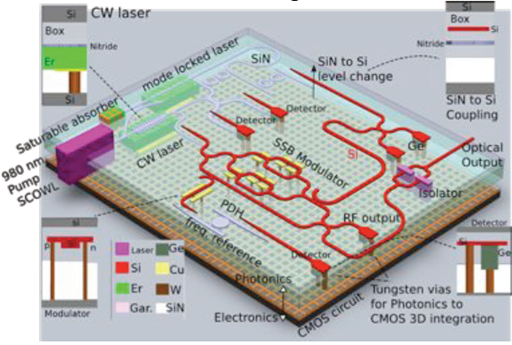
\includegraphics[width=13cm]{figures/ephi_proposal.png} 
		\caption{\label{fig:electrical_model}Ephi proposal.}	
		\end{center}
    \vspace{-10pt}
\end{figure}

	\begin{equation}
Delay = \frac{R_0}{W} \cdot \left[C_g \cdot \chi \cdot W + C_w + C_{eff} \right] + R_{mod} \cdot C_{eff}
	\label{eqn:delay}
	\end{equation}	
	
%%	
%%\section{A General Modulator Driver Model}
%%
%%	
%%
%%The generalized driver model is shown in Figure \ref{fig:electrical_model} as an inverter 
%%chain pre-driver followed by a final driver stage.  The final driver stage is attached to the modulator device, and drives the device to voltage $V_a$.  There is some parasitic capacitance associated with the wiring device, $C_{w}$.  To the first order, the diode itself (if in the reverse-bias regime) can be approximated as a series resistance $R_{mod}$ and a reverse-bias capacitance $C_{mod,Va}$. 
%%
%%The circuit topology of the final drive stage should be chosen based on whether the driver is for a carrier-injection or carrier-depletion device, and it will also change depending on the diode drive voltage $V_a$ compared to the process $V_{DD}$.  For the carrier-depletion case, if $V_a < V_{DD}$, a low-swing topology can be used (Figure \ref{fig:electrical_model}a); 
%%otherwise a voltage-boosting circuit may be necessary (Figure \ref{fig:electrical_model}b).  
%%In both cases, the final stage can be modeled as an effective resistance $R_{eff}$ and a parasitic capacitance $C_{par}$.
%%
%%The $R_{eff}$ will change with the width $W$ of the final drive transistors as $R_0/W$.  $C_{par}$ is dominated by the gate capacitance of the final drive transistors.  Because electron mobility is typically twice that of hole mobility, PMOS transistors tend to be sized twice as large as their counterpart NMOS, making the total width $3 \cdot W$.  $C_{par}$ is modeled as $3 \cdot W \cdot \gamma \cdot C_g$, with $C_g = 1$ fF/$u$m in the process and $\gamma = C_d/C_g$. 
%%
%%The final stage must be sized such that the target charge $Q$ is achieved on $C_{eff}$ in less than a bit-time.  Logical effort analysis is used to determine an appropriate size for the driver's width ($W$) and pre-driver chain fan-out ($FO$) to meet the data rate requirements. 
%%
%%
%%%	\begin{equation}
%%%Delay = \frac{R_0}{W} \cdot \left[C_g \cdot \chi \cdot W + C_w + C_{eff} \right] + R_{mod} \cdot C_{eff}
%%%	\label{eqn:delay}
%%%	\end{equation}
%%
%%The $CV^2$ energy-per-bit of the final driver stage can be calculated based on its parasitic capacitance $C_{par}$, taking into consideration that for random data with 50\% ones and zeros, a zero-to-one transition (a charging of that capacitance) will only happen 1/4 of the time.  The ``$V^2$'' term in $CV^2$ will depend on whether the final driver stage is a low-swing or a boost driver.  In the case of a low-swing driver, $C_{par}$ is only charged to $V_a$ with the energy coming from $V_{DD}$ (thus $V_a \cdot V_{DD}$ equaling the ``$V^2$'' term); in the case of a boost driver, the ``$V^2$'' term is equal to $V_a^2$.  
%%
%%	\begin{equation}
%%E_{dr} = \frac{C_{par} + C_{w}}{4} \cdot \mbox{max} \left(V_a \cdot V_{DD}, V_a^2 \right) + \frac{1}{4} \cdot \frac{3 \cdot C_g \cdot W}{1 - \frac{1}{FO}} \cdot V_{DD}^2
%%	\label{eqn:delay}
%%	\end{equation}
%%
%%
%%	\begin{figure}[H]\begin{center}
%%    \vspace{-20pt}
%%		\subfloat[Driver energy cost $E_{dr}$.]{\label{fig:Edr_vs_dr}
%%			\includegraphics[width=6cm]{fig/Edr_vs_dr.eps}}
%%		\subfloat[Total modulator energy cost $E_{mod,tot}=E_{ms}+E_{dr}$.]{\label{fig:Etot_vs_dr}
%%			\includegraphics[width=6cm]{fig//Etot2_vs_dr.eps} }
%%		\caption{Energy costs to reach the target $ER_{dB}=6$ dB for various values of $IL_{dB}$.\label{fig:energy}}
%%    \vspace{-10pt}
%%	\end{center} \end{figure}
%%	
%%
%%Figure \ref{fig:energy} shows the driver energy-per-bit cost to 
%%reach $ER_{dB}=$ 6 dB for various values of $IL_{dB}$.  For current 
%%modulator device technology, to satisfy data rates up to 30 Gb/s, 
%%the intrinsic RC time constant of the device allows designers to 
%%choose $R_{mod}$ up to 1 k$\Omega$ without significant energy penalty, relaxing the modulator optical losses due to contact placement.  Verifying this theoretical model with measured results is one goal of this thesis.
%%
%%
%%
%%\section{Carrier Injection Modulator Driver}
%%
%%The double-data-rate modulator driver is designed as a configurable all-digital push-pull driver circuit with sub-bit-time pre-emphasis and split supplies, operating over the wide range of drive currents required for the variety of optical devices. 
%%%The driver is configured for experiments with and without active carrier depletion. 
%%The split power supply and level-shift drivers allow tradeoffs between energy efficiency and extinction ratio without increasing the power consumption of the back-end.  Unlike previous work on sub-bit pre-emphasis \cite{xu_osa07}, where different voltage values are used to pre-emphasize the modulator drive, in this work we change the on-resistance of the modulator driver connected to a fixed supply voltage.  A novel signal conditioning technique allows the driver circuit to achieve an open eye from the modulator device at roughly 10x the intrinsic bandwidth of the device.
%%
%%\subsection{A Case for Pre-Emphasis}
%%
%%A pre-emphasized topology is used for the carrier-injection modulator driver.  This design decision was made by first analyzing a simplified driver model, shown in Figure \ref{fig:diode_simple}, to gain a basic understanding of the limits and requirements of the circuit.  It is assumed that we have chosen a target extinction ratio (3 dB is a minimum choice) and a minimum $\Delta N_0 = 2.1\e{18}$ cm$^{-3}$ necessary to reach that extinction ratio. 
%%The minimum injected charge necessary is $\Delta Q_0 = 1.9\e{-13}$ C for a ring modulator in an IBM 45 nm process with $L_j$ = 6 $\mu$m, $r$ = 8 $\mu$m, and a target extinction ratio of 3 dB at $\lambda_0$ = 1200 nm.
%%
%%	\begin{figure}[H]
%%		\begin{center}
%%			\includegraphics[width=7cm]{fig/diode_simple.eps}
%%			\caption{\label{fig:diode_simple}First order charge rise time schematic.}
%%		\end{center}
%%	\end{figure}
%%
%%
%%The charge $Q(t)$ in the I-region follows a first-order linear differential equation, where $i(t)$ is the diode current and $\tau_c$ is the carrier lifetime in the I-region \cite{pierret}.
%%	\begin{equation}
%%\frac{dQ(t)}{dt} = i(t) - \frac{Q(t)}{\tau_c}
%%	\label{eqn:dq-dt}
%%	\end{equation}
%%
%%The solution to this equation makes the initial condition assumption that \mbox{$Q(0) = 0$}.  $Q_S$ is the steady-state charge in the I-region.
%%
%%	\begin{equation}
%%Q(t) = Q_S \Big[ 1 - e^{-\frac{t}{\tau_c}}\Big]
%%	\end{equation}
%%
%%	\begin{equation}
%%Q_S = \tau_c \cdot i(t)
%%	\end{equation}
%%
%%The nonlinear relationship between the charge in the I-region and the optical transmissivity can be exploited to increase energy efficiency and speed.  With a fixed driver resistance, on a transition from a 0 to a 1 bit, the charge in the I-region will steadily grow toward $Q_S$, reaching $Q_S$ perhaps sometime in the middle of the bit.  If the driver circuit provides $i(t)$ such that $Q_S = Q_0$, the resulting optical eye diagram will be poor at high speed due to the slow rising trajectory of $Q(t)$.  A sub-bittime pre-emphasized driver can do much better \cite{kern_vlsi07}.  A  driver with a much lower resistance for a small portion of the bit time on a 0 to 1 transition will increase the charge in the I-region much more rapidly, improving the optical eye diagram \cite{xu_osa07}.  The total driver resistance during pre-emphasis is referred to as $R_A$, the resistance during the remaining forward bias portion of the bit time is $R_B$, and the reverse-bias driver resistance is $R_C$.
%%
%%
%%This pre-emphasis technique has three main advantages:
%%
%%\begin{itemize} 
%%\item It lowers the amount of steady-state charge necessary for a `1'-bit, increasing energy effeciency.
%%\item Because the amount of steady-state charge has been reduced, there is less chance of shifting all the way to the next optical channel.
%%\item The modulator can operate at higher speeds due to an improved eye as in Figure \ref{fig:eye}.
%%\end{itemize}
%%
%%	\begin{figure}[H]
%%		\begin{center}
%%		\subfloat[Without pre-emphasis]{\label{fig:eye_nopreemp}\includegraphics[width=7cm]{fig/eye_nopreemp.eps}}
%%		\subfloat[With pre-emphasis]{\label{fig:eye_preemp}\includegraphics[width=7cm]{fig/eye_preemp.eps}}\\
%%		\caption{\label{fig:eye} A simulation demonstrating how pre-emphasis can improve eye quality, raising the bitrate (1 ns carrier lifetime on random data).}
%%		\end{center}
%%	\end{figure}
%%
%%To estimate the required driver resistance at a datarate of 2 Gb/s, it is assumed that the pre-emphasis driver will be active for the first quarter of a bit time for a zero-to-one transition, or 50 ps.  The goal of the pre-emphasis driver will be to raise $Q(t)$ by $\Delta Q_0$ by the end of the pre-emphasis pulse.  The minority carrier lifetime, $\tau_c$, is between 1-2ns in the IBM 45nm process.
%%
%%	\begin{equation}
%%Q(t = 50 \, \mbox{ps}) = Q_0 = Q_{SA} \cdot (1 - e^{(-50 \, \mbox{ps} / 10 \, \mbox{ns})})
%%	\end{equation}
%%
%%	\begin{equation}
%%Q_{SA} = 3.9\e{-12} \, \mbox{C}
%%	\end{equation}
%%
%%
%%
%%$Q_{SA}$ is approximately 20x the steady-state charge, indicating that the transient current should be ~20x larger than the steady-state.  In a commercial CMOS process, $V_{DD}$ is fixed, and is approximately \mbox{1.0 V} at the 45 nm node.  A digital driver circuit can be approximated to the first order by the circuit shown in Figure \ref{fig:diode_simple}.  $R_{dr}$ is the total resistance of the driving transistors and $R_S$ is the series resistance of the P-I-N diode.  This simplification of the driver circuit is used to find an appropriate starting range for the driver resistance to make a first estimate at the transistor sizing.  
%%
%%
%%
%%
%%The high $V_{th}$ of the P-I-N diode means that a low $R_S$ and $R_{dr}$ are necessary to achieve a reasonable $Q_S$.  The $V_{th}$ of the modulator diode is measured as approximately 0.8 V for currents in the range of 1 mA.  The $V_{DD}$ limit of the process is also a concern.  For demonstrating short-term functionalality of the modulator driver, $V_{DD}$ can be temporarily raised to 1.5 or 2.0 V if the driver cannot provide enough current at 1.0 V.  This solution is not feasible for mainstream adoption of silicon photonics due to the degradated reliability of the circuits.   It is also important to note that above a certain bias voltage, the carrier concentration in the I-region begins to saturate, as shown in Figure \ref{fig:n-v_sentaurus}, so increasing the voltage further may have little effect.
%%
%%	\begin{equation}
%%i(t) = \frac{V_{DD} - V_{th}}{R_{A} + R_{S}}
%%	\end{equation}
%%
%%	\begin{equation}
%%Q_{SA} = \tau_c \cdot \frac{V_{DD} - V_{th}}{R_{A} + R_S}
%%	\end{equation}
%%
%%	\begin{equation}
%%R_A + R_S = \tau_c \cdot \frac{V_{DD} - V_{th}}{Q_{SA}} = 51 \Omega
%%	\end{equation}
%%
%%With a diode contact resistance of approximately 30 $\Omega$, the pre-emphasis driver resistance should be 20 $\Omega$.  Unfortunately, due to the high $V_{th}$, the transistors are likely to be in the triode region, and this target is difficult to achieve without an unreasonably large driver circuit.  In the first generation of circuits we opt to raise the supply locally to 1.5 V, which relaxes the output driver requirements to at least $R_A$ = 150 $\Omega$. In practice, the goals can be achieved with even larger output impedance since at above a supply voltage of 1.2 V, the driver is mostly in saturation during the transition and acts more as a current source.
%%
%%Once the pre-emphasis pulse ends and the charge reaches the level of $Q_0$, the pre-emphasis driver will deactivate and the forward-bias driver will be active.  The forward-bias driver will only sustain the charge at the level of $Q_0$.
%%
%%	\begin{equation}
%%R_B  = \tau_c \cdot \frac{V_{DD} - V_{th}}{Q_{0}} - R_S = 1.0 k \Omega
%%	\end{equation}
%%
%%The forward-bias driver resistance is much more reasonable.  We chose a nominal design point where the pre-emphasis driver is four times the strength of the forward-bias driver and two times the strength of the reverse-bias driver.  This is just an approximate analysis to provide the design intuition. 
%%
%%	\begin{figure}[H]
%%		\begin{center}
%%			\includegraphics[width=10cm]{fig/loadline.eps}
%%			\caption{\label{fig:loadline}Load line showing pre-emphasis driver and forward-bias driver.}
%%		\end{center}
%%	\end{figure}
%%
%%
%%
%%
%%%[talking about eos1; obsolete] The chip has eight standalone modulator drivers based on our best estimate of the diode properties.  These eight modulators are the only electronics on the chip and are confined to the top row; the rest is dedicated solely to optical test structures.  
%%
%%\subsection{Carrier-Injection Driver Circuit}
%%
%%	The modulator driver circuit is a custom digital push-pull circuit with sub-bittime pre-emphasis \cite{moss_isscc13}.  Two on-chip 31-bit pseudo-random-bit-sequence (PRBS) generators feed the double-data-rate (DDR) driver circuit (the PRBS generators are now shown in the schematic).   The schematic for the driver is shown in Figure \ref{fig:eos12_fb_driver_schematic}.  The circuit has four parallel drive segments, named segments A, B, C, and D.  Each segment is responsible for either forward- or reverse-biasing the P-I-N diode depending on the appropriate drive regime.  The strength of these drive segments can be digitally tuned across four bits.  The inset in the schematic shows the logic levels of the control signals for each segment in the case of a 0-1-0 data pattern.
%%
%%	\begin{figure}[H]
%%		\begin{center}
%%			\includegraphics[width=14cm]{fig/eos12_fb_driver_schematic/eos12_fb_driver_schematic.eps}
%%			\caption{\label{fig:eos12_fb_driver_schematic}Conceptual schematic of the EOS-series carrier injection modulator driver.}
%%		\end{center}
%%	\end{figure}
%%
%%
%%Figure \ref{fig:eos12_fb_driver_schematic_shaded_AB} illustrates which segments are active at the beginning of a zero to one transition. Both the sub-bittime forward-bias driver (Segment A) and the full-bittime forward-bias driver (Segment B) are active, maximizing the current into the I region.  Segment A is activated by a tunable delay element.
%%
%%	\begin{figure}[H]
%%		\begin{center}
%%			\includegraphics[width=14cm]{fig/eos12_fb_driver_schematic/eos12_fb_driver_schematic_shaded_AB.eps}
%%			\caption{\label{fig:eos12_fb_driver_schematic_shaded_AB}Conceptual schematic of the EOS-series carrier injection modulator driver. Segments A and B are active at the beginning of a 0-1-bit transition.}
%%		\end{center}
%%	\end{figure}
%%
%%After a short time (less than a bit time), Segment A deactivates, while Segment B remains on for the duration of the one-bit, lowering the current into the diode.  This is shown in Figure \ref{fig:eos12_fb_driver_schematic_shaded_B}.   
%%
%%	\begin{figure}[H]
%%		\begin{center}
%%			\includegraphics[width=14cm]{fig/eos12_fb_driver_schematic/eos12_fb_driver_schematic_shaded_B.eps}
%%			\caption{\label{fig:eos12_fb_driver_schematic_shaded_B}Conceptual schematic of the EOS-series carrier injection modulator driver. Segment B is active for the full duration of a 1-bit.}
%%		\end{center}
%%	\end{figure}
%%
%%Figure \ref{fig:eos12_fb_driver_schematic_shaded_C} illustrates the beginning of a one-to-zero transition.  Segment C is active, reverse-biasing the diode and sweeping the injected carriers out of the intristic region of the P-I-N diode for the first portion of the zero-bit.
%%
%%	\begin{figure}[H]
%%		\begin{center}
%%			\includegraphics[width=14cm]{fig/eos12_fb_driver_schematic/eos12_fb_driver_schematic_shaded_C.eps}
%%			\caption{\label{fig:eos12_fb_driver_schematic_shaded_C}Conceptual schematic of the EOS-series carrier injection modulator driver. Segment C is active at the beginning of a 1-0 transition, reverse-biasing the diode and sweeping carriers out of the intrinsic region.}
%%		\end{center}
%%	\end{figure}
%%
%%Figure \ref{fig:eos12_fb_driver_schematic_shaded_D} shows how Segment C deactivates, and Segment D activates, for the duration of a zero-bit after the pre-emphasis pulse.  Reverse-biasing the diode at this stage would be the traditional method to use.  However, note that Segment D is actually \emph{forward-biasing} the diode, rather than reverse-biasing it.  Segment D forward-biases the diode slightly below the diode's threshold voltage.  This pre-charges the diode for a fast zero-to-one transition.  It also takes advantage of the nonlinear relationship between the charge in the I-region and optical transmissivity.  By forward-biasing the diode slightly below threshold, the charge inside the I-region is not sufficient to change the device's optical transmissivity; in a sense, it is below the optical threshold of the device.  This novel technique was published in ISSCC \cite{moss_isscc13}.
%%
%%
%%	\begin{figure}[H]
%%		\begin{center}
%%			\includegraphics[width=14cm]{fig/eos12_fb_driver_schematic/eos12_fb_driver_schematic_shaded_D.eps}
%%			\caption{\label{fig:eos12_fb_driver_schematic_shaded_D}Conceptual schematic of the EOS-series carrier injection modulator driver. Segment D is active for the duration of a 0-bit after the pre-emphasis pulse has ended.  The weak forward bias pre-charges the P-I-N diode without changing the optical logic state.}
%%		\end{center}
%%	\end{figure}
%%
%%
%%Each segment has been designed as a DAC, where control bits can configure the strength of the segment via the digital back-end.  Some of the configurable elements of the pre-emphasis profile are seen in Figure \ref{fig:preemp_profile}.  The unpredictable diode parameters such as carrier lifetime prompted a highly configurable design to account for process uncertainty, and the difficulty of coupling high-speed signals in the 1 to 10 GHz range on- and off- chip lead us to develop a sophisticated on-chip digital backend infrastructure.  The wide range of configurability will be able to adapt to the uncertain device properties of the P-I-N diode.  The carrier lifetime of the poly-Si is unpredictable due to an unknown amount of defects and varies from fab to fab, so this parameter was difficult to estimate during design of the first generation of the circuit, but the minority carrier lifetime of the silicon estimated to be between the ranges of 100 ps and 2 ns.  It was later measured to be 1 ns.  Simulations suggest the modulator can also work at 10 Gb/s if the minority carrier lifetime were shorter; the operation of the modulator depends heavily on the carrier lifetime.  The driver currents for pre-emphasis, forward bias, and reverse bias can be tuned to within an order of magnitude.  The duration of the pre-emphasis pulse can be tuned in the range of 10 ps to 100 ps.
%%
%%
%%	\begin{figure}[H]
%%		\begin{center}
%%			\subfloat[Pre-emphasis varying]{\label{fig:preemp_a}\includegraphics[width=3.5cm]{fig/preemp_profile_a.eps}}
%%			\subfloat[Forward-bias varying]{\label{fig:preemp_b}\includegraphics[width=3.5cm]{fig/preemp_profile_b.eps}}
%%			\subfloat[Reverse-bias varying]{\label{fig:preemp_c}\includegraphics[width=3.5cm]{fig/preemp_profile_c.eps}}
%%			\subfloat[Pulse width varying]{\label{fig:preemp_d}\includegraphics[width=3.5cm]{fig/preemp_profile_d.eps}}
%%		\end{center}
%%		\caption{\label{fig:preemp_profile}Configurable parameters of the P-I-N current profile.}
%%	\end{figure}
%%
%%
%%	\begin{figure}[H]
%%		\begin{center}
%%			\includegraphics[width=10cm]{fig/eos12_fb_driver_schematic/eos12_driver_heads.eps}
%%			\caption{\label{fig:eos12_driver_heads}Carrier injection driver final DCVS driver heads}
%%		\end{center}
%%	\end{figure}
%%
%%%\ v0: make this larger, multiple per row
%%
%% There are additional delay elements not shown in the schematic which can help tune the arrival of data transitions to the final stage to correct for manufacturing variation.  These delay elements are also digitally configurable across four bits each.  The delay element consists of a current-starved inverter, shown in Figure \ref{fig:delay}
%%	\begin{figure}[H]
%%		\begin{center}
%%			\includegraphics[height=6cm]{fig/delay.eps}
%%			\caption{\label{fig:delay}Delay element schematic}
%%		\end{center}
%%	\end{figure}
%%
%%
%%	\begin{figure}[H]
%%		\begin{center}
%%			\includegraphics[width=16cm]{fig/eos4_bowtie.eps}
%%			\caption{\label{fig:eos4_bowtie}Micrograph of carrier-injection modulator driver and device.}
%%		\end{center}
%%	\end{figure}
%%
%%
%%
%%
%%%	\begin{figure}[H]
%%%		\begin{center}
%%%			\subfloat[Forward-bias segment]{\label{fig:eos4_dcvs_fb}\includegraphics[width=7cm]{fig/eos4_dcvs_fb.eps}}
%%%			\subfloat[Reverse-bias segment]{\label{fig:eos4_dcvs_rb}\includegraphics[width=7cm]{fig/eos4_dcvs_rb.eps}}
%%%		\end{center}
%%%		\caption{\label{fig:eos4_dcvs}Final driver stage: DCVS NAND gates}
%%%	\end{figure}
%%
%%The final stage of the EOS4 driver is a set of segmented differential cascade voltage switched (DCVS) NAND gates.  These DCVS gates are connected to an isolated power rail, $HV_{DD}$, so that the drive voltage of the final stage of the driver can be increased above the process voltage of 1.0 V without risking damage to other transistors on the die.  There are three sets of segmented DCVS NAND gates; one set is for the preemphasis, one set is for forward-biasing the diode for a full bit period, and the final set is for reverse-biasing the diode for a full bit period.  The schematics for these forward and reverse-bias DCVS NAND gates is shown in Figure \ref{fig:eos12_driver_heads}.
%%
%%
%%%	%\begin{landscape}
%%%	\begin{figure}[H]
%%%		\begin{center}
%%%			\includegraphics[width=14cm]{fig/eos8_modulator_fb_schematic.eps}
%%%			\caption{\label{fig:eos4_modulator_full}Full schematic of injection-based modulator driver.}
%%%		\end{center}
%%%	\end{figure}
%%%	%\end{landscape}
%%
%%
%%
%%In addition to modulators, this chip also has configurable data receivers, configurable clock receivers, and data snapshot buffers.  A serial scan chain allows the bits to be set and read easily by an FPGA or a similar external circuit.  A micrograph of the modulator design is shown in Figure \ref{fig:eos4_bowtie}.
%%
%%
%%\subsection{Advantages of Signal Conditioning}
%%
%%The signal conditioning technique mentioned in the previous section helps to overcome the inherent bandwidth limitation of the device.  The device's electrical 3 dB bandwidth, shown in Figure \ref{fig:eos12_device} in the previous chapter, is limited to approximately 250 MHz due to the minority carrier lifetime of the device.  A traditional ``unconditioned'' pre-emphasis profile is shown in Figure \ref{fig:eos12_step_response}a.  In the unconditioned profile, there is a strong forward-bias pre-emphasis at the beginning of a zero-to-one transition, and a strong reverse-bias pre-emphasis at a one-to-zero transition.  After the strong reverse-bias pre-emphasis, a weaker reverse-bias persists for the duration of the zero-bit.
%%
%%
%%	\begin{figure}[H]
%%		\begin{center}
%%			\subfloat[Unconditioned]{\label{fig:eos12_strength_profile_unconditioned}\includegraphics[width=7cm]{fig/eos12_strength_profile/eos12_strength_profile_unconditioned.eps}}\\
%%			\subfloat[Conditioned]{\label{fig:eos12_strength_profile_conditioned}\includegraphics[width=7cm]{fig/eos12_strength_profile/eos12_strength_profile_conditioned.eps}}
%%		\end{center}
%%		\caption{\label{fig:eos12_profile}EOS12 pre-emphasis profile, unconditioned and conditioned }
%%	\end{figure}
%%
%%In the conditioned case, shown in Figure \ref{fig:eos12_profile}b, the profile differs for a zero-bit.  After a one-to-zero transition, there is still a strong reverse-bias pre-emphasis to sweep the carriers out of the P-I-N diode's intrinsic region, snapping the ring back to its unbiased state.  After the pre-emphasis pulse is over, the circuit slightly forward-biases the diode as a pre-charge for the next one-to-zero transition.  This trick helps to overcome the bandwidth limitations on a zero-to-one transition caused by the long minority carrier lifetime.
%%
%%The impact of this technique can be seen in Figure \ref{fig:eos12_step_response}.  The zero-to-one and one-to-zero step responses are measured and normalized in the Y-axis for fair comparison.  In the unconditioned case, the zero-to-one transition is significantly slower.  
%%	\begin{figure}[H]
%%		\begin{center}
%%			\subfloat[Unconditioned]{\label{fig:eos12_step_response_unconditioned}\includegraphics[width=10cm]{fig/eos12_step_response/eos12_step_response_unconditioned.eps}}\\
%%			\subfloat[Conditioned]{\label{fig:eos12_step_response_conditioned}\includegraphics[width=10cm]{fig/eos12_step_response/eos12_step_response_conditioned.eps}}
%%		\end{center}
%%		\caption{\label{fig:eos12_step_response}EOS12 Step Response, unconditioned and conditioned}
%%	\end{figure}
%%
%%
%%In the conditioned case, the rising and falling edges are nicely matched, which will provide the most open eye and thus the optimal performance.
%%
%%
%%
%%\subsection{Experimental Test Setup}
%%
%%
%%	\begin{figure}[ht]
%%		\begin{center}
%%			\includegraphics[height=8cm]{fig/lab_setup/table_setup.eps}
%%			\caption{\label{fig:table_setup}Table setup}
%%		\end{center}
%%	\end{figure}
%%
%%	Our test station consists of an optical table with an infrared camera on a vertically-mounted microscope.   Custom fiber holders have been machined and on each side of the die, a fiber holder sits atop a computer-controlled 5-axis stage.  A second horizontally-mounted camera behind the die allows us to easily see how close the fiber is to the surface.  The packaged die plugs into a custom circiuit board containing level shifters for the scan chain signals and current DACs to power the polysilicon heaters.  %A novel "bowtie" tunable modulator which is less sensitive to waveguide loss has also been fabricated.  
%%
%%
%%For experiments from chip-to-chip, a dual-table setup has been created with a trans-lab fiber running underneath the table.
%%	\begin{figure}[ht]
%%		\begin{center}
%%			\includegraphics[height=6cm]{fig/lab_setup/dual_setup.eps}
%%			\caption{\label{fig:dual_setup}Dual-chip setup}
%%		\end{center}
%%	\end{figure}
%%
%%
%%\subsection{Experimental Results}
%%	  The most significant result thus far is a demonstration of working modulator devices in both the 1550 nm band and the 1280 nm band.  The optical eye diagrams shown in the following subsections demonstrate the first measured monolithically integrated modulator driver in a convenitonal CMOS process.  The speed of the driver, and thus the eye width, is limited largely by the carrier lifetime.  The eye height for 1280 nm results are worse than comparable 1550 nm results due to the lack of an optical amplifier in the 1280 nm band.  The noise of the optical oscilloscope significantly worsened the eye height as well.
%%
%%\subsubsection{Without Signal Conditioning}
%%Previous generations of the carrier-injection modulator driver without signal conditioning reached maximum speeds of approximately 600 Mbps and were published in Optics Express 2012 \cite{orcutt_optex12}.  The eye diagrams at 1550nm (reaching 600 Mbps) and 1280nm (reaching 250 Mbps) are shown in Figure \ref{fig:eye_diagrams}.  The only reason the 1550nm result is at a higher datarate is because we were able to supply more optical power at that band, which resulted in a more open eye.
%%
%%	\begin{figure}[H]
%%		\begin{center}
%%			\subfloat[1550 nm eye diagram at 600 Mbps]{\label{fig:eye_1550}\includegraphics[width=6cm]{fig/carrier_injection_eye_diagrams/eye_eos8p102_1550_600mb_prbs.eps}}
%%			\subfloat[1280 nm eye diagram at 250 Mbps]{\label{fig:eye_1280}\includegraphics[width=6cm]{fig/carrier_injection_eye_diagrams/eye_eos8p103_cell214_250Mbps_noc.eps}}
%%		\end{center}
%%		\caption{\label{fig:eye_diagrams}Optical eye diagrams of the injection-based modulator driver.}
%%	\end{figure}
%%
%%The measured electrical power and extinction ratio of the modulator \emph{without} signal conditioning is shown in Figure \ref{fig:isscc12_emi_vs_dr}.  This generation of the design can achieve an open eye at 250 Mbps at approximately 4pJ/bit at an extinction ratio of around 2.3 dB.
%%
%%	\begin{figure}[H]
%%		\begin{center}
%%			\includegraphics[width=10cm]{fig/isscc12_emi_vs_dr/isscc12_emi_vs_dr.eps}
%%			\caption{\label{fig:isscc12_emi_vs_dr}Measured electrical power of 1280 nm injection-based modulator}
%%		\end{center}
%%	\end{figure}
%%
%%
%%%	\begin{figure}[H]
%%%		\begin{center}
%%%			\includegraphics[height=6cm]{fig/step_response/step_response_214.eps}
%%%			\caption{\label{fig:step_response}Measured optical step response of 1280nm injection-based modulator \fixme{}}
%%%		\end{center}
%%%	\end{figure}
%%
%%\vspace{-2em}
%%\subsubsection{With Signal Conditioning}
%%
%%With the signal conditioning described in this section, performance increased considerably.  Virtually the same circuit, with only minor changes to implement the improved pre-emphasis profile, was able to boost performance to the multi-gigabit regime, reaching 2.5 Gb/s, shown in Figure \ref{fig:eye_eos12_2p5gbps}.  This result was published in ISSCC 2013 \cite{moss_isscc13}.  This result is the fastest, most energy-efficient carrier-injection modulator in a sub-100nm monolithically-integrated CMOS process to date.
%%
%%	\begin{figure}[H]
%%		\begin{center}
%%			\includegraphics[width=9cm]{fig/carrier_injection_eye_diagrams/eye_eos12_2p5gbps.eps}
%%			\caption{\label{fig:eye_eos12_2p5gbps}Optical 2.5 Gb/s eye diagram of signal-conditioned EOS carrier-injection modulator at 1550 nm}
%%		\end{center}
%%	\end{figure}
%%
%%The energy-efficiency and extinction ratio achieved by the signal-conditioned EOS carrier-injection modulator is shown in Figure \ref{fig:isscc13_emi_vs_dr}. This iteration of the design achieved 1.23 pJ/b at an extinction ratio of 3.4 dB at 2.5 Gb/s.
%%
%%	\begin{figure}[H]
%%		\begin{center}
%%			\includegraphics[width=11cm]{fig/isscc13_emi_vs_dr/isscc13_emi_vs_dr.eps}
%%			\caption{\label{fig:isscc13_emi_vs_dr}Measured electrical power of signal-conditioned EOS carrier-injection modulator at 1550 nm}
%%		\end{center}
%%	\end{figure}
%%
%%The energy-efficiency improves with speed because the on-current through the forward-bias diode gets amortized over a larger number of bits.
%%
%%This concludes the analysis of the carrier-injection modulator.
%%
%%\section{Depletion-Mode Modulator Drivers}
%%
%%The carrier-injection modulator in the previous section has two main drawbacks.  First, its energy efficiency is low due to the need to forward-bias the P-I-N diode for each one-bit.  Secondly, the minority carrier lifetime of the diode limits the speed of the device to low-Gb/s speeds.
%%
%%The depletion-mode modulator device does not have these drawbacks.  Rather than forward-biasing the diode structure to inject free carriers, the diode structure is reverse-biased to increase the size of the depletion region.  In contrast to the carrier-injection device, the depletion-mode device is more sensitive to the process doping levels and material properties, and depending on the exact device behavior, may require higher reverse-bias voltages (beyond the native process $V_{DD}$).  However, as a topology, the depletion-mode modulator has far more potential in terms of speed and energy-efficiency than the carrier-injection approach.
%%
%%\subsection{Design Constraints}
%%From the analysis in Chapter 2, we concluded that a reverse-bias drive voltage of $V_a = 2.0$ V is necessary to reach the required $\Delta Q$ for a 1-0 transition (in the lab, the device performed better than expected and its performance is satisfactory at 1.5 V).  For a 0-1 transition, the driver circuit also needs a forward-bias conduction path.  In a modern CMOS process, $V_{DD}$ is limited to 1.0 V, and adding an extra supply rail is impractical, leading us to consider charge-pump based circuits.
%%
%%Additionally, to avoid reducing the lifespan of the driver circuit through oxide breakdown, each transistor must satisfy:
%%
%%
%%\begin{itemize} 
%%\item $V_{ds} \le 1.0$ V
%%\item $V_{gd} \le 1.0$ V
%%\item $V_{gs} \le 1.0$ V
%%\end{itemize}
%%
%%This design constraint can be mitigated by using thicker-oxide devices for the final drive transistors; however, these transitors may impose a speed constraint.  Two driver designs are analyzed; first, a charge-pump-based approach, for reverse-bias drive voltages above 1.5V, and second, a simpler DCVS NAND-gate approach with thick-oxide final stage transistors.
%%
%%\subsection{Processor (EOS) Platform: Charge-Pump Carrier-Depletion Driver Circuit}
%%
%%	\begin{figure}[H]
%%		\begin{center}
%%			\includegraphics[height=11cm]{fig/eos8_rb_schematic/eos8_rb_schematic.eps}
%%			\caption{\label{fig:eos8_rb_schematic}Depletion-mode driver schematic}
%%		\end{center}
%%	\end{figure}
%%
%%The first depletion-mode driver design is a charge-pump circuit intended for modulator devices requiring a drive voltage much greater than the native process VDD.
%%The full schematic for the depletion-mode driver is shown in Figure \ref{fig:eos8_rb_schematic}.  An inverter chain, shown at the top of the schematic, is used to generate auxiliary data signals used at various points throughout the circuit: $\overline{data}$ represents a slightly delayed, inverted \emph{data}, \emph{data'} is a delayed version of \emph{data}, and so forth.  This circuit has two modes of operation depending on whether the current bit (\emph{data} on the schematic) is a 1 or a 0.  
%%
%%
%%	\begin{figure}[H]
%%		\begin{center}
%%			\includegraphics[height=11cm]{fig/eos8_rb_schematic/eos8_rb_schematic_forward.eps}
%%			\caption{\label{fig:eos8_rb_schematic_forward}Depletion-mode driver schematic - 1 bit - forward bias}
%%		\end{center}
%%	\end{figure}
%%
%%If the current bit is a 1, two things are happening simultaneously.  The modulator diode is being forward-biased thorugh $M_1$, $M_3$, $M_{13}$, $M_{14}$, $M_4$, and $M_2$.  The amount of forward-bias current that the driver can sustain can be digitally adjusted by the six configuration bits, labeled as \emph{en\textless5:0\textgreater} on the schematic.  At the same time, capacitors $C_1$ and $C_3$, and capacitors $C_2$ and $C_4$ are connected in parallel to share charge.  Both $C_4$ and $C_3$ were pre-charged to 1.0 V in the circuit's other state, to be described shortly.  In its steady state of operation, and after charge-sharing, both $C_1$ and $C_2$ will have reached nearly 1.0 V.  This state is shown in Figure \ref{fig:eos8_rb_schematic_reverse}.  Inactive transistors are greyed out.  
%%
%%
%%	\begin{figure}[H]
%%		\begin{center}
%%			\includegraphics[height=11cm]{fig/eos8_rb_schematic/eos8_rb_schematic_reverse.eps}
%%			\caption{\label{fig:eos8_rb_schematic_reverse}Depletion-mode driver schematic - 0 bit}
%%		\end{center}
%%	\end{figure}
%%
%%
%%	\begin{figure}[H]
%%		\begin{center}
%%			\includegraphics[height=6cm]{fig/eos8_modulator_10G_250b_prbs_montecarlo.eps}
%%			\caption{\label{fig:eos8_rb_eye}Simulated depletion-mode modulator driver eye diagram at 10 Gb/s, Monte Carlo simulation on a pseudo-random data sequence}
%%		\end{center}
%%	\end{figure}
%%
%%
%%If the current bit is a 0, again, two processes happen simultaneously.  $C_1$ and $C_2$ had previously been charged to ~1.0 V in the circuit's other state of operation.  Now they are used to reverse-bias the diode, as shown in Figure \ref{fig:eos8_rb_schematic_reverse}.  $C_1$ is pushed below $M_{15}$ to pull node $v_{ANODE}$ to -1.0 V.  Similarly, $C_2$ is stacked on top of $M_{16}$ to push node $v_{CATHODE}$ to +2.0 V.  At slow speeds, this circuit will reverse-bias the modulator diode at voltages above 2.5 V.  At its maximum speed of 10 Gb/s, the circuit can reverse-bias the diode near 2.0 V.  A simulated eye diagram is shown in Figure \ref{fig:eos8_rb_eye}.
%%
%%
%%
%%
%%The two level shifters shown in the full schematic (Figure \ref{fig:eos8_rb_schematic}) are necessary to bias transistors $M_{21}$ and $M_{22}$ to satisfy the oxide-breakdown voltage constraints.
%%
%%\subsection{Processor (EOS) Platform: DCVS-NAND Thick-Oxide Carrier-Depletion Driver Circuit}
%%
%%The second carrier-depletion design topology is intended for modulator devices which can operate with reverse-bias voltages in the 1.0 to 1.5 V range (at or slightly above the process VDD).  This transmitter circuit shown in  (Figure \ref{fig:eos16_rb_schematic} consists of a carrier-depletion optical ring resonant modulator and a 65µm x 30µm driver circuit. 
%%
%%	\begin{figure}[H]
%%		\begin{center}
%%			\includegraphics[width=14cm]{fig/eos16_rb_schematic/eos16_rb_schematic.eps}
%%			\caption{\label{fig:eos16_rb_schematic}DCVS-NAND Thick-Oxide Carrier-Depletion Driver Circuit}
%%		\end{center}
%%	\end{figure}
%%
%% In the driver, a 2-to-1 serializer performs muxing of a 2-bit input digital bitstream, a DCVS NAND-gate level-shifts the bits from VDD to the HVDD, and a final inverter in the HVDD domain drives the cathode terminal of the modulator diode. The diode anode is shorted to VSS, and the circuit applies a voltage of -HVDD to 0V across the diode for carrier-depletion operation. Based on the voltage swing requirements of our previously demonstrated devices \cite{shainline_opticsletters13}, we built both the DCVS NAND-gate and final inverter using thick-oxide transistors. Though slower, this allows HVDD to be increased well above the nominal process voltage of 1V - a precautionary measure taken to accommodate depletion modulator designs that often require higher driver voltages \cite{buckwalter_jssc12} \cite{zheng_ptl12}. 
%%
%%The optical modulator device is a lateral junction modulator [4], with interdigitated junction definition enabled by the advanced 45nm process lithography. The modulator has a free-spectral-range of 2.74 THz and optimized coupling resulting in a measured Q-factor of approximately 14,000. Given such high Q, we note that above-nominal supply voltages are unnecessary for this improved device; a swing of just -0.7V to 0V captures greater than 8dB of extinction. Thus, both the thick-oxide devices and the level-shifter can be eliminated in the future to improve speed and energy.
%%
%%	\begin{figure}[H]
%%		\begin{center}
%%			\includegraphics[width=14cm]{fig/isscc14_cmos_modulator/isscc14_cmos_modulator.eps}
%%			\caption{\label{fig:isscc14_cmos_modulator} DCVS-NAND Thick-Oxide Modulator Energy and Eye Diagrams}
%%		\end{center}
%%	\end{figure}
%%
%%
%%Figure \ref{fig:isscc14_cmos_modulator} shows modulator eye diagrams taken at 2 Gb/s and 3.5 Gb/s. The centers of the eyes are bit-error free for 1012 bits, verified using an external TIA-to-FPGA-based bit-error-rate test. A layout error resulting in delay-imbalanced 0-to-1 and 1-to-0 paths through the thick-oxide DCVS NAND gate causes the distorted eye shape and ultimately limits the maximum achievable data-rate of the driver. Higher HVDD is required at higher data-rates solely for improving rise and fall times limited by the slow thick-oxide devices in the driver circuit. With appropriate supply scaling, the energy-cost of the driver scales gracefully from 20 fJ/bit at 2 Gb/s (VDD of 0.8V and HVDD of 0.8V) to 70 fJ/bit at 3.5 Gb/s (VDD of 1.0V and HVDD of 1.2V). The depletion modulator's reverse-bias operation and digital driver implementation result in flat energy-cost vs. data-rate, and provide more than an order of magnitude better energy-efficiency compared to the forward-bias injection modulator demonstrated previously in the same process \cite{moss_isscc13}. 
%%
%%
%%\subsection{Memory (Micron) Platform: Carrier-Depletion Driver Circuit}
%%The circuit for the Micron platform, shown in Figure \ref{fig:micron_schematic} does not require the thick-oxide transistors necessary in the EOS platform due to the higher native process VDD.  For this reason, a voltage-limiting additional NMOS transistor is added to the final stage.
%%
%%The backend interfaces with the custom TX and RX heads through 8-to-2 mux/demux tree SerDes and runs at one-fourth the data clock. The custom transmit head performs the final 2-to-1 serialization, and is designed to interface with a variety of integrated photonic modulators.
%%
%%	\begin{figure}[H]
%%		\begin{center}
%%			\includegraphics[width=14cm]{fig/micron/micron_schematic.eps}
%%			\caption{\label{fig:micron_schematic} Micron modulator driver schematic.}
%%		\end{center}
%%	\end{figure}
%%
%%
%%	\begin{figure}[H]
%%		\begin{center}
%%			\includegraphics[width=14cm]{fig/micron/micron_micrograph.eps}
%%			\caption{\label{fig:micron_micrograph} Micrograph of Micron modulator device.}
%%		\end{center}
%%	\end{figure}
%%
%%
%%The DDR modulator circuit is a push-pull diode driver with an NMOS pull-up on the device anode to limit the forward-bias voltage. The depletion-mode ridge microring modulator (shown in Figure \ref{fig:micron_micrograph} has simple geometry that can be electrically contacted without introducing loss to the optical mode. It is created via a partial polySi etch and doped to form a pn-junction across the ridge. The circuit drives the junction to -VDD for a full-depletion logic 1 and VREF-VT for a weak forward-bias 0, modulating the depletion region width. This creates a shift in resonance from the carrier-plasma effect and modulates the input wavelength.
%%
%%
%%
%%	\begin{figure}[H]
%%		\begin{center}
%%			\includegraphics[width=14cm]{fig/micron/micron_energy.eps}
%%			\caption{\label{fig:micron_energy} Energy-per-bit of the Micron modulator driver.}
%%		\end{center}
%%	\end{figure}
%%
%%
%%
%%The ridge modulator and circuit energy-per-bit vs. data-rate tradeoffs are shown in Figure \ref{fig:micron_energy}.  To our knowledge, this chip demonstrated the first chip-to-chip monolithically-integrated photonic link in a bulk CMOS process, demonstrating that photonic interconnects need not be confined to niche, high-cost processes. Dense and energy-efficient photonic interconnects are feasible even on cost-aware mainstream bulk CMOS platforms. 
%%
%%%\fixme{The system chips described in the previous chapter were designed in a commercial IBM 45 nm thin-SOI process.  Its 3 mm x 3 mm$^2$ area is divided into horizontal test rows containing various optical test structures, such as vertical grating couplers, paperclip loss measurement structures, waveguides of different widths, photodiodes, and modulators.  A minimal number of Design Rule Check (DRC) waivers were necessary to tape out the design, proving that the technology is compatible with existing processes.}
%%
%%\section{EPHI}
%%
%%Although the focus of this thesis is on \emph{monolithically}-integrated silicon photonics, in parallel, we taped out a chip in a hybrid flow where a photonics chip is wafer-level-bonded to a dedicated CMOS chip, named EPHI.
%%
%%During EPHI chip design, a family of modulator drivers were created to cover a wide range of process uncertainties at design time, to provide drive functionality for a family of modulator devices, and also to provide backup testing capability for various testing scenarios.
%%
%%The primary modulator driver design is a 50$\mu$m x 50$\mu$m double-data-rate (DDR) driver circuit, shown in Figure \ref{fig:ephi_modulator_schematic}.  The driver is connected to an optical modulator device.  The optical modulator device is a lateral junction modulator, leveraging the Soref electro-optical effect in silicon to electrically control the resonant frequency of the modulator ring’s resonance.   The driver circuit moves the optical modulator’s resonance into and out of the laser wavelength channel to modulate the light.  The driver circuit modulates the modulator diode depletion width by varying the reverse-bias voltage across the device’s diode contacts; through the Soref electro-optic effect, this depletion width change causes an optical resonance shift.  This driver circuit is designed to drive a wide family of optical devices. The final stage consists of a level-shifting inverter on the modulator device’s cathode, where the gate of the NMOS pull-up device is connected to a voltage reference circuit (labeled VREF).   The modulator diode junction is driven to VREF-Vt for a weak forward-bias, providing additional modulator extinction by further shrinking the junction’s depletion region.  During full depletion, the modulator diode junction is reverse-biased to –VDD.  
%%
%%
%%	\begin{figure}[ht]
%%		\begin{center}
%%			\includegraphics[width=14cm]{fig/ephi/modulator_schematic.eps}
%%			\caption{\label{fig:ephi_modulator_schematic}The EPHI DDR modulator driver}
%%		\end{center}
%%	\end{figure}
%%
%%
%%
%%	\begin{figure}[ht]
%%		\begin{center}
%%			\includegraphics[width=10cm]{fig/ephi/ephi_5gbps_extracted_moddriver_eye.eps}
%%			\caption{\label{fig:ephi_5gbps_extracted_moddriver_eye}Extracted eye diagram of the modulator driver output (with 20fF load) at 5 Gbps.}
%%		\end{center}
%%	\end{figure}
%% 
%%The modulator is fed by the digital back-end, where two PRBS generators operating at 2.5 Gb/s provide two data streams, shown in Figure 6 as IN[0] and IN[1].  A pre-driver block multiplexes these two data streams into a single 5 Gb/s data stream, carefully controlling the clock domains through the use of two flip-flops and a latch.  The predriver block also buffers these signals to ensure that the fan-out is appropriate to drive the final driver head.
%% 
%%
%%	\begin{figure}[ht]
%%		\begin{center}
%%			\includegraphics[width=12cm]{fig/ephi/moddriver_layout.eps}
%%			\caption{\label{fig:ephi_moddriver_layout}The 50 $\mu$m x 50 $\mu$m modulator driver.}
%%		\end{center}
%%	\end{figure}
%%
%%The layout of the modulator circuit is shown in Figure 8.  The 50$\mu$m x 50$\mu$m layout consists of approximately 60\% decoupling capacitors.
%% 	A simplified modulator driver variant was also created, shown in Figure \ref{fig:ephi_lite_modulator}.  This driver does not have the ability to drive the modulator junction into a weak forward bias, so the optical extinction will suffer; however, if the optical device has a high extinction, this design will be more energy-efficient and the lower extinction may not matter.   In this variant, the anode of the modulator device is connected to VSS, and the cathode is connected to a buffered inverter standard-cell.  This design is very simple and robust and should be able to drive modulator devices with capacitances in the range of 20-40fF at 5 Gb/s.
%%
%%	\begin{figure}[ht]
%%		\begin{center}
%%			\includegraphics[width=14cm]{fig/ephi/lite_modulator.eps}
%%			\caption{\label{fig:ephi_lite_modulator}Simplified modulator driver.}
%%		\end{center}
%%	\end{figure}
%%
%%A third variant, an “ultralite” modulator driver, is shown in Figure \ref{fig:ephi_ultralite_modulator}.  This design is simply a 4x-sized inverter, with an input capacitance of approximately 2.4 fF.  This driver is a more extreme design because the final inverter will only be able to drive modulator devices at 5 Gb/s if the total device capacitance is under 10 fF, which is below expectations.  However, if the device capacitance is low, this will be an extremely low-power design.  The final inverter is connected to a separate power grid (AVDD) from the pre-driver so that the final drive power can be directly measured, separate from the pre-driver and digital backend.
%%
%%	\begin{figure}[ht]
%%		\begin{center}
%%			\includegraphics[width=14cm]{fig/ephi/ultralite_modulator.eps}
%%			\caption{\label{fig:ephi_ultralite_modulator}``Ultralite'' modulator driver.}
%%		\end{center}
%%	\end{figure}
%%
%% 
%%The digital backend is a complex place-and-routed block, and although it is verified through simulation and other verification tools, it does rely on high transistor yield to operate properly.  Given that the process is under development, backup designs that can operate independently from the digital backend were created so that the modulator driver can be tested in the event of a digital backend failure.
%%Figure \ref{fig:cml2cmos_modulator} shows the schematic for the independent backup modulator driver.  The final drive head, described earlier, is now fed by a CML-to-CMOS converter rather than the digital backend and predriver.  The CML (current-mode-logic) inputs are fed directly from GSG pads.  Low-voltage-swing CML inputs are used to boost the operating speed to 5 Gb/s.  The three-stage CML-to-CMOS converter converts these 200mV differential swings into a single full-rail CMOS swing at the date output.  The CML-to-CMOS final stage is buffered appropriately to directly drive the final drive head without an additional pre-driver.
%% 
%%	\begin{figure}[ht]
%%		\begin{center}
%%			\includegraphics[width=14cm]{fig/ephi/cml2cmos_modulator.eps}
%%			\caption{\label{fig:cml2cmos_modulator}Modulator driver, fed directly from a CML-to-CMOS converter.}
%%		\end{center}
%%	\end{figure}
%%
%%
%% 
%%	\begin{figure}[ht]
%%		\begin{center}
%%			\includegraphics[width=10cm]{fig/ephi/cml2cmos_and_moddriver_layout.eps}
%%			\caption{\label{fig:cml2cmos_and_moddriver_layout}Layout of 150µm x 50µm  CML-to-CMOS (on the left) and modulator driver (on the right).}
%%		\end{center}
%%	\end{figure}
%%
%%
%%
%%This same backup approach of attaching a CML-to-CMOS converter is also used for the ``lite'' and ``ultralite'' variants, as shown in Figures \ref{fig:ephi_lite_cml2cmos_modulator} and \ref{fig:ephi_ultralite_cml2cmos_modulator}. 
%%
%% 
%%	\begin{figure}[ht]
%%		\begin{center}
%%			\includegraphics[width=14cm]{fig/ephi/lite_cml2cmos_modulator.eps}
%%			\caption{\label{fig:ephi_lite_cml2cmos_modulator}CML-to-CMOS converter attached to the “lite” inverter-based modulator driver.}
%%		\end{center}
%%	\end{figure}
%%
%%
%% 
%%	\begin{figure}[ht]
%%		\begin{center}
%%			\includegraphics[width=14cm]{fig/ephi/ultralite_cml2cmos_modulator.eps}
%%			\caption{\label{fig:ephi_ultralite_cml2cmos_modulator}CML-to-CMOS converter attached to the “ultralite” single-inverter driver.}
%%		\end{center}
%%	\end{figure}
%%
%%The Ephi modulator driver designs, from the perspective of the focus of this thesis, were a peripheral exploration into the hybrid wafer-level bonding topology presented in Chapter 1.  
%%
%%\section{Conclusion}
%%
%%
%%This chapter used the analysis from Chapter 2 to implement modulator driver circuits for both the carrier-injection and carrier-depletion device topologies.  These designs were taped-out and tested in the lab, providing breakthrough results, and showing the importance of close interaction between device- and circuit-designers.  This work provides the main contribution of this thesis, through the demonstration of the fastest, most energy-efficient monolithically-integrated modulator and driver circuit in a sub-100nm to date.  
%%
%To implement these circuits in a sub-100nm thin-SOI CMOS process, some postprocessing steps had to be performed on the die after they came back from the foundry.  The next chapter will explain these steps in fine detail. 


\appendix
\chapter{Tables}

\begin{table}
\caption{Armadillos}
\label{arm:table}
\begin{center}
\begin{tabular}{||l|l||}\hline
Armadillos & are \\\hline
our	   & friends \\\hline
\end{tabular}
\end{center}
\end{table}

\clearpage
\newpage

\chapter{Figures}

\vspace*{-3in}

\begin{figure}
\vspace{2.4in}
\caption{Armadillo slaying lawyer.}
\label{arm:fig1}
\end{figure}
\clearpage
\newpage

\begin{figure}
\vspace{2.4in}
\caption{Armadillo eradicating national debt.}
\label{arm:fig2}
\end{figure}
\clearpage
\newpage

%% This defines the bibliography file (main.bib) and the bibliography style.
%% If you want to create a bibliography file by hand, change the contents of
%% this file to a `thebibliography' environment.  For more information 
%% see section 4.3 of the LaTeX manual.
\begin{singlespace}
\bibliography{main}
\bibliographystyle{plain}
\end{singlespace}

\end{document}

